\documentclass{article}

\usepackage{amsmath,amsfonts,amsthm,amssymb,amsbsy,amstext,amscd,amsxtra,multicol,mathtools}
\usepackage{mathtext}

\usepackage[T2A]{fontenc}
\usepackage[utf8]{inputenc}
\usepackage[english,russian]{babel}
\usepackage{textcomp}
\usepackage{graphicx}
\graphicspath{ {./images/} }
\usepackage{float}
\usepackage{color}
% \usepackage{xspace}
% \usepackage[document]{ragged2e}
% \usepackage{multirow}
\usepackage{indentfirst}
% \usepackage{verbatim}
\usepackage{tikz}
% \usepackage{forest}

% Выделенное поле для примечаний
\usepackage[most]{tcolorbox}
\definecolor{block-gray}{gray}{0.90} % уровень прозрачности (1 - максимум)
\newtcolorbox{myquote}{colback=block-gray, grow to right by=0mm, grow to left by=0mm,
boxrule=0pt,boxsep=0pt,breakable} % настройки области с изменённым фоном

\setlength{\parindent}{0.8cm}
\setlength{\parskip}{0cm}

\def\eps{\varepsilon}
\usepackage[left =2cm, right=2cm, top=2cm, bottom=2cm, bindingoffset=0cm]{geometry}

% Настройка секций (внутрення нумерация, номер не отображается)
\renewcommand{\thesection}{}
\renewcommand{\thesubsection}{\arabic{section}.\arabic{subsection}}
\makeatletter
\def\@seccntformat#1{\csname #1ignore\expandafter\endcsname\csname the#1\endcsname\quad}
\let\sectionignore\@gobbletwo
\let\latex@numberline\numberline
\def\numberline#1{\if\relax#1\relax\else\latex@numberline{#1}\fi}
\makeatother

\usepackage{hyperref}% http://ctan.org/pkg/hyperref
\hypersetup{%
  colorlinks = true,
  linkcolor  = black
}





\begin{document}

\author{Лабунец Л.В. \& Паймин Антон}
\title{Нейронные сети. Лекции.}

\makeatletter
\begin{center}
    {\fontsize{14pt}{24pt}\selectfont\bfseries\@title\par}
    {\fontsize{14pt}{16pt}\@author\par}
\end{center}
\makeatother

\tableofcontents
\newpage

% \setcounter{section}{4}
\section{Лекция}

\subsection{Математическая модель многослойного перцептрона}

Рассмотрим на примере 3-слойной архитектуры (в количество слоёв входят только слои, реализующие нелинейное отображение).
Рассмотрим сигналы, поступающие на вход нейронов, но для избежания путаницы, будем визуализировать связи только для первых нейронов соответствующих слоёв.
Рассмотрим эти связи и соотв. им параметры.

\begin{figure}[htbp]
    \centering
    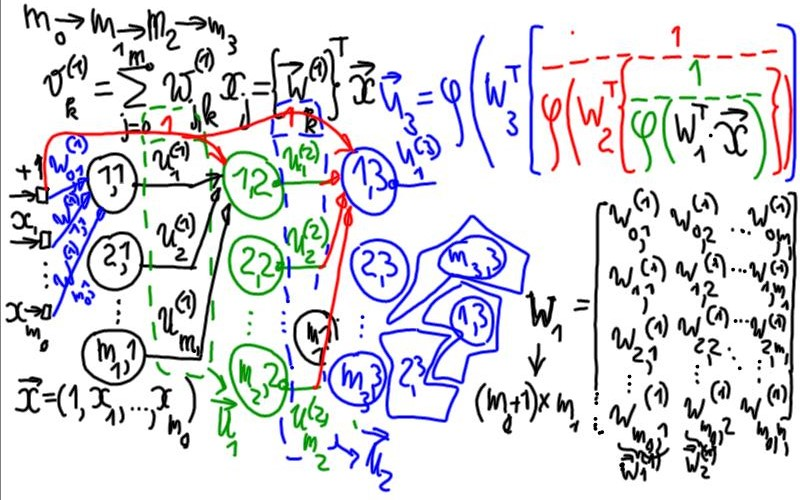
\includegraphics[width=\textwidth]{hyperflat_3_1.jpeg}
    \caption{Структура многослойного перцептрона}
    \label{hyperflat_3_1}
\end{figure}

3-слойный перцептрон содержит 0-й слой - слой источников (черные квадратики). 
Имеется $m_{0}$ входов, на которые поступают признаки $\vec{x} = (1, x_0, ..., x_{m_{0}})$, 3 скрытых слоя.

Примем следующие правила индексации скрытых нейронов и нейронов выходного слоя:
первый эл-т индекса - номер нейрона, второй - номер слоя: $m_{i,j}$  - $i$-й нейрон $j$-го скрытого слоя.

Выпишем веса нейронов $i$-го слоя в виде матрицы $W_i$, столбец которой $\vec{w}_i^{(k)}$ является вектором весов $i$-го нейрона $k$-го слоя.
Количество строк матрицы - количество входов слоя + 1 (на вход поступает расширенный вектор), количество столбцов - количество нейронов слоя.
Элемент матрицы $w_{i,j}^{(k)}$ - вес $i$-го входа $j$-го нейрона $k$-го слоя.
У первого скрытого слоя имеется $m_0$ входов (слой источников) и он содержит $m_1$ нейронов.

\begin{equation}
    W_1 = 
    \begin{pmatrix}
        w_{0,1}^{(1)} & w_{0,2}^{(1)} & \dots & w_{0,{m_1}}^{(1)} \\
        w_{1,1}^{(1)} & w_{1,2}^{(1)} & \dots & w_{1,{m_1}}^{(1)} \\
        w_{2,1}^{(1)} & w_{2,2}^{(1)} & \dots & w_{2,{m_1}}^{(1)} \\
        \vdots        & \vdots        & \ddots & \vdots           \\
        w_{{m_0},1}^{(1)} & w_{{m_0},2}^{(1)} & \dots & w_{{m_0},{m_1}}^{(1)} \\
    \end{pmatrix}
\end{equation}

Рассмотрим первый слой.
На вход каждого нейрона слоя поступает сигнал смещения $+1$, взвешиваемый \textit{биасом} $w_{0,i}^{(1)}$. 
Также на вход этого нейрона поступают входные признаки $x_i$, взвешиваемые \textit{синаптическими весами} $w_{1,j}^{(1)}$ до $w_{{m_0},j}^{(1)}$ - веса $i$-го признака $j$-го нейрона в первом слое.   
Для экономии места введём вектор синаптических весов конкретного нейрона:

\begin{equation}
    \vec{w}_j^{(k)} = 
    \begin{pmatrix}
        w_{0,j}^{(k)} & w_{1,j}^{(k)} & \dots & w_{{m_0},j}^{(k)}
    \end{pmatrix}
    ^T
\end{equation}


Индекс в скобках - номер слоя, нижний индекс - номер нейрона. Т.е., $\vec{w}_1^{(1)}$ - вектор синаптических весов 1-го нейрона 1-го слоя.

На выходе $i$-го нейрона $k$-го слоя формируется сигнал $u_i^{(k)}$. 
Выпишем формулу для вычисления сигнала на выходе 1-го нейрона 1-го слоя $u_1^{(1)}$. Опять, в скобках - номер слоя, индекс - номер нейрона.
Для этого необходимо посчитать сигнал на выходе сумматора $k$-го нейрона (\textit{индуцированного локального поля}):

\begin{myquote}
    \textit{Не очень удачно были выбраны индексы, но оставил, как на презентации}
\end{myquote}

\begin{equation}
    {v}_k^{(1)} = \sum_{j=0}^{m_0} w_{j,k}^{(1)} \cdot x_j = [\vec{w}_{k}^{(1)}]^T \cdot \vec{x}
\end{equation}


\begin{equation*}
    {v}_2^{(1)} = [\vec{w}_{2}^{(1)}]^T \cdot \vec{x}
\end{equation*}

где $j$ - номер нейрона, $k$ - номер слоя, $w_{j,k}^{(1)}$ - компоненты ..., $\vec{x}$ - расширенный вектор.

Из приведённых выражений можем получить общее: $W_k^T \cdot \vec{x}$ - совокупность элементов на выходе сумматоров всех нейронов $k$-го слоя.

Полученные на выходе сумматора значения подвергаются нелинейному преобразованию с помощью функции активации $\varphi(W_k^T \cdot \vec{x})$. Получаем совокупность сигналов на выходе функций активации нейронов. 
Для первого слоя: $\varphi(W_1^T \cdot \vec{x})$, для второго: $\varphi(W_2^T \cdot \vec{x})$ и т.д.

Для получения из матрицы $W_1$ матрицы $W_2$ рисуем таблицу:

\begin{center}
    Количество входов и выходов скрытых слоёв (без учёта "расширенности" векторов):

    \begin{tabular}{c | c |  c | c |}
        & 1 слой & 2 слой & 3 слой \\
        \hline
        Количество входов  & $m_0$ & $m_1$ & $m_2$ \\
        \hline
        Количество выходов & $m_1$ & $m_2$ & $m_3$ \\
        \hline
    \end{tabular}
\end{center}

Выпишем матрицу $W_2$;
\begin{equation}
    W_1 = 
    \begin{pmatrix}
        w_{0,1}^{(2)} & w_{0,2}^{(2)} & \dots & w_{0,{m_2}}^{(2)} \\
        w_{1,1}^{(2)} & w_{1,2}^{(2)} & \dots & w_{1,{m_2}}^{(2)} \\
        w_{2,1}^{(2)} & w_{2,2}^{(2)} & \dots & w_{2,{m_2}}^{(2)} \\
        \vdots        & \vdots        & \ddots & \vdots           \\
        w_{{m_1},1}^{(2)} & w_{{m_1},2}^{(2)} & \dots & w_{{m_1},{m_2}}^{(2)} \\
    \end{pmatrix}
\end{equation}

И получим выходы сумматоров нейронов второго слоя:

\begin{myquote}
    Починить расширенные вектора!
\end{myquote}

\begin{equation}
    \vec{u}_2 = W_2^T \cdot [\dfrac{1}{\varphi(W_1^T \cdot \vec{x})}]
\end{equation}


В формуле 1 в якобы числителе - добавленный первый элемент, чтобы получить расширенный вектор-столбец.

\begin{equation}
    \vec{u}_3 = \varphi(W_3^T[\dfrac{1}{\varphi(W_2^T \cdot [\dfrac{1}{\varphi(W_1^T \cdot \vec{x})}])}])
\end{equation}

Для 4-го слоя получим:

\begin{myquote}
    \textit{Выписать матрицу с рисунка для 4 слоя, поправить формулу и выписать её}
\end{myquote}

Увеличение слоёв нецелесообразно из-за рекурсивной структуры модели многослойного перцептрона (последовательность вложенных блоков),
что приводит к уменьшению скорости вычисления, увеличению занимаемой памяти и накопления ошибок.
Также по мере увеличения параметров модели, возникает \textit{эффект переобучения}, а по мере увеличения количества слоёв, количество параметров увеличивается экспоненциально.

Возможно применение альтернативных архитектур - например, сети радиальных базисных функций.
Также необходимо применение методов регуляризации, например, метод \textit{хирургии мозга} - исключения из каждого слоя неинформативных нейронов или целых слоёв.
Существуют методы обучения, подразумевающие цикличность. Более детально см. "Нейронные сети. Полный курс" Саймона Хайкина (?).

Также существует теорема, доказанная Колмогоровым, утв., что многомерная скалярная функция может воспроизводить любую закономерность сколь угодно большой сложности. Теорема об универсальной аппроксимации многослойным перцептроном, утв., что архитектура многослойного перцептрона \textit{теоретически} позволяет с любой заданной точностью синтезировать
многомерную по количеству входов векторную функцию, что позволяет строить модели нелинейных дискриминантных границ в пространстве признаков и, соотв., определять принадлежность
данных кластерам. 




\subsection{Системный подход к синтезу алгоритмов обучения многослойного перцептрона}

\begin{figure}[htbp]
    \centering
    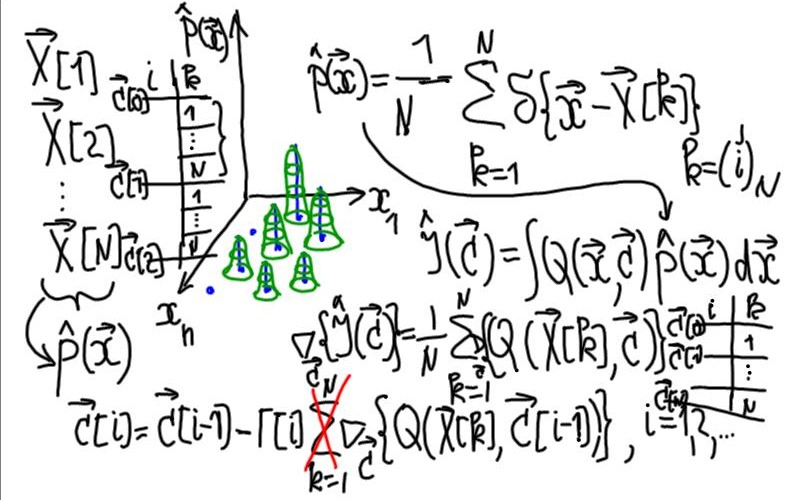
\includegraphics[height=10 cm]{hyperflat_5_1.jpeg}
    \caption{Системный подход к обучению многослойного перцептрона}
    \label{hyperflat_5_1}
\end{figure}

Согласно системному подходу к синтезу алгоритмов обучения многослойного перцептрона, необходимо выполнить 3 шага:
\begin{enumerate}
    \item Выбор цели обучения;
    \item Оценка градиента средних потерь целевой функции по параметрам нейронной сети;
    \item Использование алгоритмом поиска оптимальных параметров.
\end{enumerate}

Предполагается наличие функционала качества работы системы, оптимальное значение которого и ищется.

\begin{figure}[htbp]
    \centering
    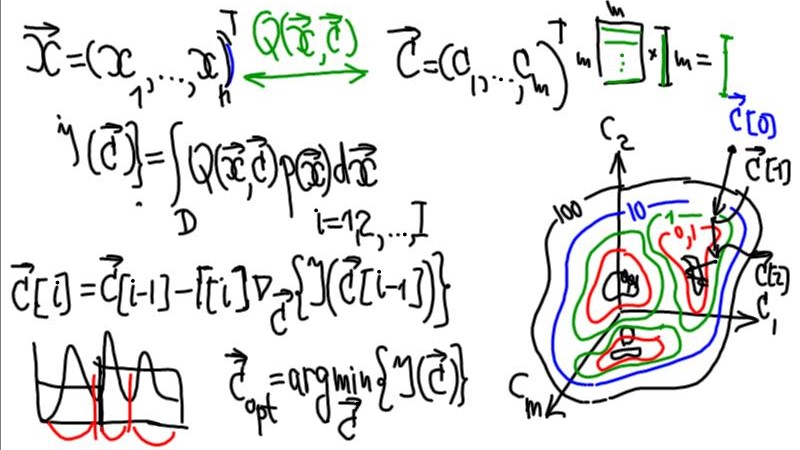
\includegraphics[height=8 cm]{hyperflat_4_1.jpeg}
    \caption{Обучение нейронной сети}
    \label{hyperflat_4_1}
\end{figure}

Будем рассматривать 3 объекта анализа
\begin{enumerate}
    \item Пространство входных воздействий $\vec{x}$ - сигналы, поступающие на вход системы (обучающие и контрольные примеры), и соответствующее пространство входных воздействий, в котором существует область $D$ все возможных входных воздействий;
    \item Вектор параметров системы $\vec{C}$ и пространство, ему соответствующее, в которому существуют эквипотенциальные гиперповерхности, все точки которых соотв. определенным значениям функционала качества. Необходимо найти область мимальных/максимальных значений этого функционала качества;
    \item Функция стоимости (потерь, приобретений) $Q(\vec{x}, \vec{c})$, определяющая потери/приобретения, которые можно измерить, если на вход системы поступает воздействие $\vec{x}$, а система находится в в состоянии $\vec{C}$.
\end{enumerate}

Набор этих 3 объектов позволяет математически строго сформулировать выбор цели обучения в виде функционала средних потерь (среднего риска).
Сделать это несложно, необходимо протестировать область $D$ всех входных воздействий: зафиксировать $\vec{x}$ и выбрать параметры системы $\vec{C}$. 
Для каждого зафиксированного выбора параметров системы необходимо вычислить потери по выбранной для кажого вхожного воздействия и просуммировать их:

\begin{equation}
    J(\vec{C}) = \int_{D} Q(\vec{x}, \vec{C}) p(\vec{x}) d\vec{x}
\end{equation}

Полученное $J(\vec{C})$ - средний риск (средние потери), $p(\vec{x})$ - весовая функция, сглаживающая аномальные значения (плотность распределения вероятностей входных воздействий).

На практике возможны 2 ситуации:
\begin{enumerate}
    \item Нетипичный случай полной априорной определённости - полное знание входных воздействий (весовой функции $p(\vec{x})$, Типа распределения и тд.);
    \item Типичный случай - функция задана набором обучающий примеров
\end{enumerate}

Во втором случае необходимо выполнить предварительную выборочную оценку весовой функции $p(\vec{x})$ по набору обучающих примеров.

Однако, будем считать весовую функцию $p(\vec{x})$ известной, тогда возможно посчитать функционал ошибок $J(\vec{C})$.

\subsection{Алгоритм обучения нейронной сети (метод градиентного поиска)}
\begin{enumerate}
    \item Выбрать начальное приближение параметров нейронной сети $\vec{C}[0]$ ($0$ - номер итерации), и оценить потери;
    \item Выбрать оптимальное направление поиска (вектор антиградиента $-\nabla\vec{C}$, указывающий направление, в котором потери убывают с максимальной скоростью);
    \item Выбрать шаг поиска (используется процедура стохастической аппроксимации Роббенса-Монро, в соответствии с которой с каждой итерацией длина шага уменьшается обратно пропорционально номеру итерации);
    \item[] В полученной точке выполняется подтверждение сходимости (сравнение итераций), вычисление нового направления и шага.
\end{enumerate}

Процедура описывается следуюшим выражением:

\begin{equation}
    \vec{C}[i] = \vec{C}[i-1] - \Gamma[i] \nabla\vec{C} \{ J(\vec{C}[i-1]) \}
\end{equation}

Цель обучения: 

\begin{equation}
    \vec{C}_{opt} = \arg \min_{\vec{C}} \{ J(\vec{C}) \}
\end{equation}

Существуют также методы, не требующие вычилсения частной производной, - метод деформируемого многоранника Нелдера-Мида (симплекс-поиск).

\begin{myquote}
    \textit{Прикладное нелинейное программирование, Химмельблау}
\end{myquote}

Обучение сводится к решению задачи оптимизации. Существуют ограничения на значения параметров системы в виде равенств или неравенств.

Результаты выполнения алгоритма зависят от выбора начального приближения, что приводит к необходимости выбора нескольких начальных приближений для обнаружения всех локальных минимумов.
Существенное преимущество в этом случае обеспечивают генетические алгоритмы.

\subsection{Алгоритм обучения нейронной сети для случая набора обучающих примеров}




\section{Дистанционная}




\section{Опоздал на полчаса}

\begin{figure}[H]
    \centering
    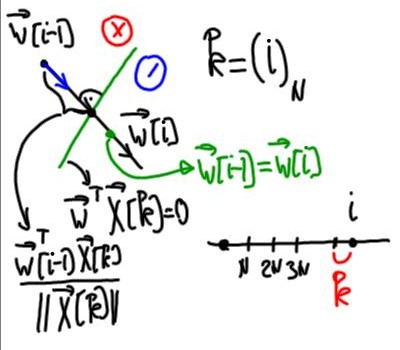
\includegraphics[height=8 cm]{hyperflat_7_1.jpeg}
    \caption{Аппроксимация многомерной скалярной функции}
    \label{hyperflat_7_1}
\end{figure}

\textbf{Геометрическая интерпретация}
Параметр скорости обучения $\eta$ выбирают, как .. 
Переходя от одного к другому обучающему примеру, приближаемся к поверхности разрезанной пирамиды.

\subsection{Пример с квадратичной функцией потерь}

\begin{figure}[htbp]
    \centering
    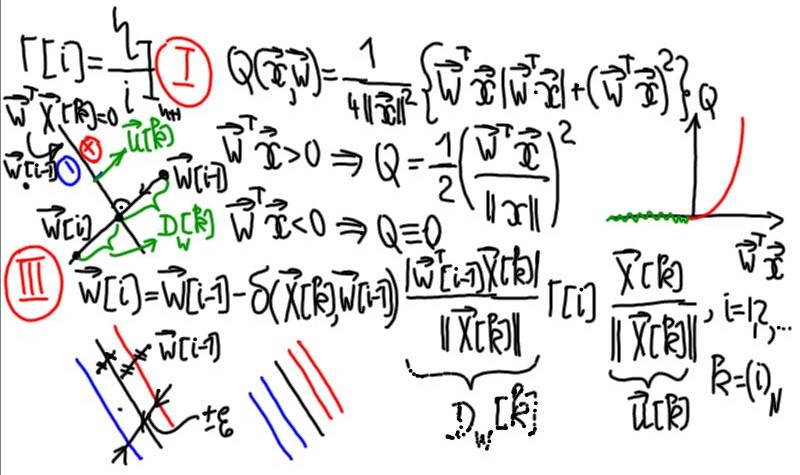
\includegraphics[height=7cm]{hyperflat_8_1.jpeg}
    \caption{\dots с квадратичной функцией потерь}
    \label{hyperflat_8_1}
\end{figure}

Фиксируем потери, пропорциональные квадрату расстояния до гиперплоскости обучающего примера, ---
потери возрастают квадратично. Методика рассмотрена на предыдущем (дистанционном) занятии.

\begin{myquote}
    \textit{Вычислить градиент функции потерь на листике}
\end{myquote}

Имея текущий обучающий пример $x_k$ и текущие параметры нейрона $\vec{W}[i-1]$,
..

В W-пространстве нормаль $\vec{u}[k]$ вычисляется как: 

\begin{equation}
    \dfrac{\vec{X}_k}{\| \vec{X}_k \|}
\end{equation}

Положим, что для $k$-го обучающего примера параметры неудачны. В этом случае опускаем перепендикуляр
к гиперплоскости и вычисляем расстояние до неё:

\begin{equation}
    D_W [k] = \dfrac{\lvert \vec{W}^T [i-1] \vec{X}[k] \rvert}{\| \vec{X}[k] \|}
\end{equation}

Долю масштаба определяют компоненты матрицы $\Gamma[i]=\dfrac{\eta}{i} I_{n\times m}$, где $I_{n \times m}$ - единичная матрица.

\begin{myquote}
    \textit{Харман, Математические основы математической вычислительной томографии, глава "РВТ"}
\end{myquote}

\begin{myquote}
    \textit{Также в книге присутствует алгоритм, в котором для гиперплоскости каждого обучающего примера выбирается некая погрешность и гиперплоскость обволакивается полосой
    шириной $\pm \varepsilon$ в связи с присутствием погрешностей в "реальных" примерах.}
\end{myquote}

Для простоты анализа здесь был выбран режим последовательного обучения, однако ранее были обсуждены также алгоритмы
\textit{смешанного обучения}.

\begin{myquote}
    \textit{Рекомендовано выписать этот алгоритм для простой и экспоненциальной (задача со звёздочкой) скользящей средней}
\end{myquote}

Здесь рассмотрен случай линейно разделимых разделимых векторов образов, исходя из предположения, что система 
линейных неравенств имеет минимум одно решение.
Иначе будет минимум одна зона в $W$-пространстве, характеризуемая количеством ошибочных классификаций 
и необходим алгоритм, строящий \textit{оптимальную гиперплоскость}.

Для \textit{оптимальной гиперплоскости} количество неизбежных ошибочных классификаций минимально. 
Такой метод был реализован Владимиров Вапником в \textit{методе опорных векторов}.

Булавский (НГУ) предложил симплекс-метод для решения несовеместных систем линейных неравенств --- 
поиска компромиссного решения. 
Метод применим для случая линейно неразделимых векторов образов и является альтернативой методу 
опорных векторов. 
Метод не получил широкого распространения, имеется только препринт.


\begin{myquote}
    \textit{Препринт есть у ЛЛВ}
\end{myquote}

\subsection{Аппроксимация многомерной скалярной функции}

\begin{figure}[htbp]
    \centering
    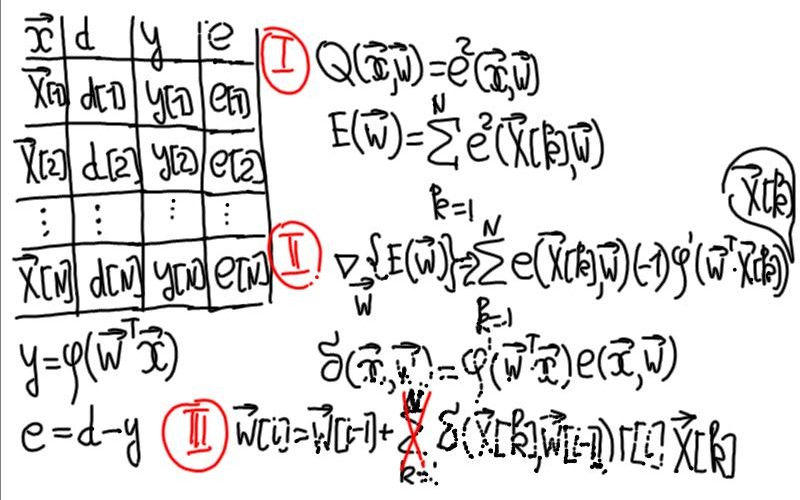
\includegraphics[height=7cm]{hyperflat_9_1.jpeg}
    \caption{Аппроксимация многомерной скалярной функции}
    \label{hyperflat_9_1}
\end{figure}

Рассмотрим альтернативную дихотомии задачу - аппроксимацию многомерной скалярной функции,  т.е.
синтез закономерности, скрытой в данных, с помощью многослойного перцептрона.
В данном случае стоит воспринимать прецептрон как устройство воспроизведения математической модели.

\begin{table}[H]
    \centering
    \begin{tabular}{| c | c | c | c |}
        \hline
        $\vec{x}$ & $d$ & $y$ & $e$ \\
        \hline
        $\vec{X}[1]$ & $d[1]$ & $y[1]$ & $e[1]$ \\
        \hline
        $\vdots$ & $\vdots$ & $\vdots$ & $\vdots$ \\
        \hline
        $\vec{X}[N]$ & $d[N]$ & $y[N]$ & $e[N]$ \\
        \hline
    \end{tabular}
    \label{table:scalar-func-table}
    \caption{Табличная форма задания многомерной скалярной функции}
\end{table}

Имеется табличная форма задания многомерной скалярной функции (\ref{table:scalar-func-table}), 
набор обучающих примеров в виде совокупности факторов (входных аргументов) $\vec{x}[i]$, $d$ ---
желаемое выходной значение скрытой закономерности, $y = \varphi (\vec{W}^T \vec{x})$ ---
фактическое значение (реакция) перцептрона и ошибка $e = d - y$.

Необходимо синтезировать математическую модель с помощью перцептронного нейрона. 
$\vec{x}$ --- обобщенный вектор образов с $+1$ в первой позиции, $\vec{W}$ ---
обобщенный вектор синаптических весов с биасом в первой позиции.

Будем выполнять задачу согласно этапам системного подхода.



\subsubsection{Выбор модели фунции стоимости}

Выберем квадратичную функцию ошибок:

\begin{equation}
    Q(\vec{x}, \vec{W}) = e^2(\vec{x}, \vec{W})
\end{equation}

Тогда средние потери будут равны:
    
\begin{equation}
    E(\vec{W}) = \sum_{k=1}^{T} e^2 (\vec{X}[k], \vec{W})
    \label{eq:sum-err}
\end{equation}



\subsubsection{Поиск градиента функции ошибок}

Необходимо найти в $W$-пространстве такую точку, которая минимизировала бы суммарную энергию ошибок $E(\vec{W})$ \ref{eq:sum-err}.

\begin{equation}
    \nabla_{\vec{W}} \{ E(\vec{W}) \} = 2 \sum_{k=1}^{N} e (\vec{X}[k], \vec{W}) \cdot (-1)
    \cdot \varphi ' (\vec{W}^T \cdot \vec{X}[k]) \vec{X}[k]
\end{equation}

В первую очередь интересно произведение первой производной функции активации и функции ошибки, 
которую обозначим $\delta(\vec{x}, \vec{W})$:

\begin{equation}
    \delta(\vec{x}, \vec{W}) = \varphi ' (\vec{W}^{T} \cdot \vec{x}) \cdot e(\vec{x}, \vec{W})
\end{equation}
\noindent
и будем называть \textit{локальным градиентом}. 
Он введён, поскольку при выполнении поиска выгоднее находиться в области ненулевых значений
функции активации (иначе итерация "пропадает").



\subsubsection{Применение алгоритма градиентного поиска}

Распишем алгоритм градиентного поиска (пакетный режим):

\begin{equation}
    \vec{W}[i] = \vec{W}[i-1] + \sum_{k=1}^{N} \delta(\vec{X}[k], \vec{W}[i-1])\cdot \vec{\Gamma[i]} \cdot \vec{X}[k]
\end{equation}

\begin{myquote}
    Рекомендовано выписывать алгоритм слева направо - скаляр, матрица, вектор.
\end{myquote}

Для усиления шумового эффекта игнорируется усреднение по всем примерам (удаление знака суммы) и выполняется 
пересчёт после каждого нового значения - последовательное обучение:

\begin{equation}
    \vec{W}[i] = \vec{W}[i-1] + \delta(\vec{X}[k], \vec{W}[i-1])\cdot \vec{\Gamma[i]} \cdot \vec{X}[k]
    \label{eq:delta-rule}
\end{equation}

Режим последовательного обучения реализует \textit{оптимизирующий алгоритм Уидроу-Хоффа} \ref{eq:delta-rule}, 
иначе называемый \textit{дельта-правилом}.

При введении сглаживания с помощью модели EMA получим \textit{обобщённое дельта-правило}.




\subsection{Алгоритм обратного распространения ошибок обучения многослойного перцептрона}

\begin{myquote}
    \textit{Lec\_neuro\_08.docx}
\end{myquote}

Основным параметром алгоритма обучения Уидроу-Хоффа является ошибка реакции, которая 
недоступна при обучении нейронов скрытых слоёв.
Эту проблему решает алгоритм обратного распространения ошибок.

Упростим схему индексации нейронов (см. \ref{hyperflat_10_1}):

\begin{figure}[htbp]
    \centering
    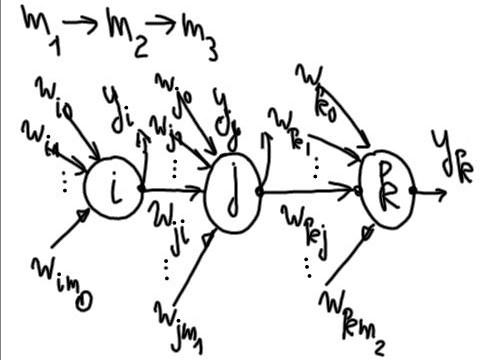
\includegraphics[width=7cm]{hyperflat_10_1.jpeg}
    \caption{1233456}
    \label{hyperflat_10_1}
\end{figure}

Для этого примем следующие соглашения:
\begin{enumerate}
    \item Для обозначения 1-го скрытого слоя используем символ $i$, нейроны 2-го скрытого слоя 
    обозначим символами $j$, выходные нейроны обозначим символами $k$, $l$ - символ линейных 
    нейронов 0-го слоя.
    \item Связь между нейронами младшего и старшего слоя (синаптический вес) --- $W{ji}$, 
    $j$ --- символ нейрона старшего слоя, $i$ --- символ нейрона младшего слоя, 
    для биаса второй индекс $0$.
    \item Во входном слое $m_0$ нейронов (функциональных входов), во 2-м слое 
    $m_1$ нейронов, в 3-м слое $m_2$ нейронов.
\end{enumerate}

Алгоритм обратного распространения содержит 2 вычислительных этапа
\begin{enumerate}
    \item \textbf{Этап прямого распространения.} В соответствии с математической моделью многослойного 
    перцептрона можем распространить все сигналы в прямом направлении --- посчитать фактические 
    реакции нейронов скрытых слоёв и выходные реакции нейронов. 
    
    В финале этого этапа обладаем выходными реакциями нейронов, на основе которых можно 
    вычислить сигналы ошибок и локальные градиенты, а значит, применить дельта-правило 
    и скорректировать параметры нейронов выходного слоя.
    \item \textbf{Этап обратного распространения.} (пунктирные линии рис 4.2 ворда). 
    На этом этапе распространяются сигналы ошибок для нейронов скрытых слоёв.
\end{enumerate}



\subsubsection{Этап прямого распространения}

Этап начинается с расчёта фактических реакций на выходе нейронов 1-го скрытого слоя. 

Рассчитаем сигнал на выходе сумматора текущего $i$-го нейрона на выходе 1-го скрытого слоя, 
на вход которого  поступает сигнал смещения "+1", взвешиваемый биасом, и входные признаки 
$x_m0$, взвешиваемые синаптическим весом $w_{im_0}$.

На выходе сумматоров получим:

\begin{equation}
    v_i (n) = \sum_{L=0}^{m_{0}} w_{il}(n) x(n)
\end{equation}

\noindent
$n$ - номер итерации.

Подвергаем его нелинейному преобразованию и получаем реакции на выходе нейронов 1-го скрытого слоя:

\begin{equation}
    y_i(n) = \varphi (v_i(n)), \quad i=\overline{1,m_1}
\end{equation}

Посчитаем сигналы на выходе сумматоров нейронов 2-го скрытого слоя:

\begin{equation}
    v_j (n) = \sum_{i=0}^{m_{1}} w_{ji}(n) y_i(n)
\end{equation}

На выходе нейронов 2-го скрытого слоя после нелийненого преобразования:

\begin{equation}
    y_j(n) = \varphi (v_j(n)), \quad j=\overline{1,m_2}
\end{equation}

Аналогично на выходе сумматоров нейронов 3-го скрытого слоя:

\begin{equation}
    v_k (n) = \sum_{j=0}^{m_{2}} w_{kj}(n) y_j(n)
\end{equation}

На выходе нейронов 3-го скрытого слоя после нелинейного преобразования:

\begin{equation}
    y_k(n) = \varphi (v_k(n)), \quad k=\overline{1,m_3}
\end{equation}

Зная фактические реакции выходных нейронов, вычислим набор ошибок:

\begin{equation}
    e_{k}(n) = d_k(n) - y_k(n)
\end{equation}

Вычисляем величину локального градиента выходных нейронов:

\begin{equation}
    \delta_k(n) = \varphi^{\prime}(v_k(n))\cdot e_k(n)
\end{equation}

Алгоритм коррекции $k$-го выходного нейрона:

\begin{equation}
    w_{kj}(n) = w_{kj}(n-1) + \dfrac{\eta}{N} \cdot \delta_{k}(n) \cdot y_j(n), k=\overline{1,m_3}
\end{equation}

Этап прямого распространения закончен.




\subsubsection{Этап обратного распространения}

В соответствии с методом потоковых графов, разработанным Станиславом Осовским и описанным в книге \glqq Нейронные сети для обработки информации\grqq,
любую сеть можно представить в виде набора графов, имеющих узлы (сигналы) и рёбра (направления распространения сигналов и коэффициенты усиления).
Если рёбра сходятся в одном узле, то это означает суммирование соответствующих сигналов.

\begin{figure}[H]
    \centering
    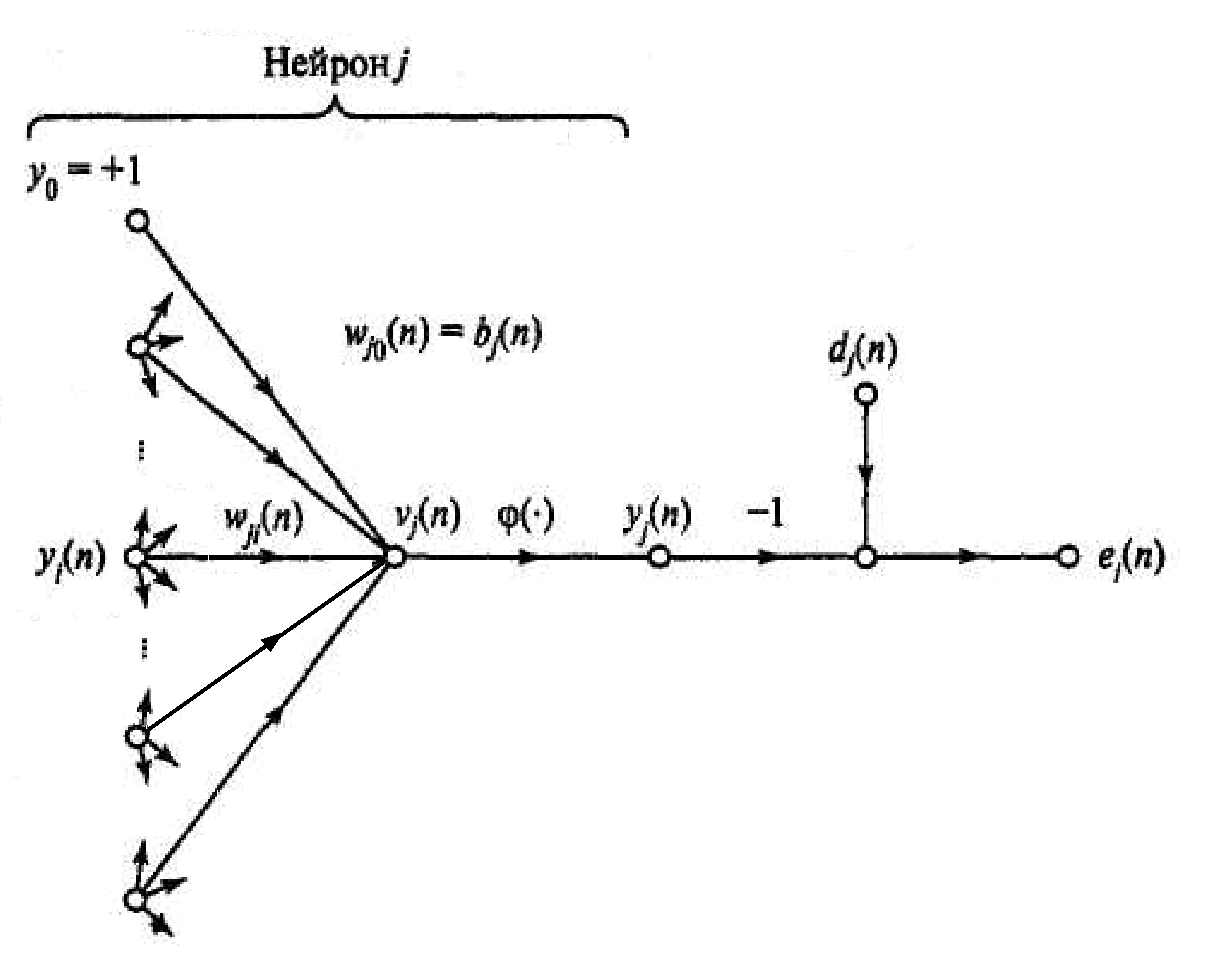
\includegraphics[height=5cm]{lec_neuro_08_4_3.png}
    \caption{Граф передачи сигнала в пределах $j$-го нейрона}
    \label{lec_neuro_08_4_3}
\end{figure}

Для нейронов выходного слоя имеем сигналы ошибки $e_1(n),\dots,e_k(n),\dots,e_{m_3}$, которые 
умножаются на вычисленные значения функции активации $\varphi^{\prime}(v_k(n))$ и получаем значения локальных градиентов 
выходных нейронов $\delta_k(n)$, а затем используем алгоритм обратного распространения ошибок.

\begin{figure}[H]
    \centering
    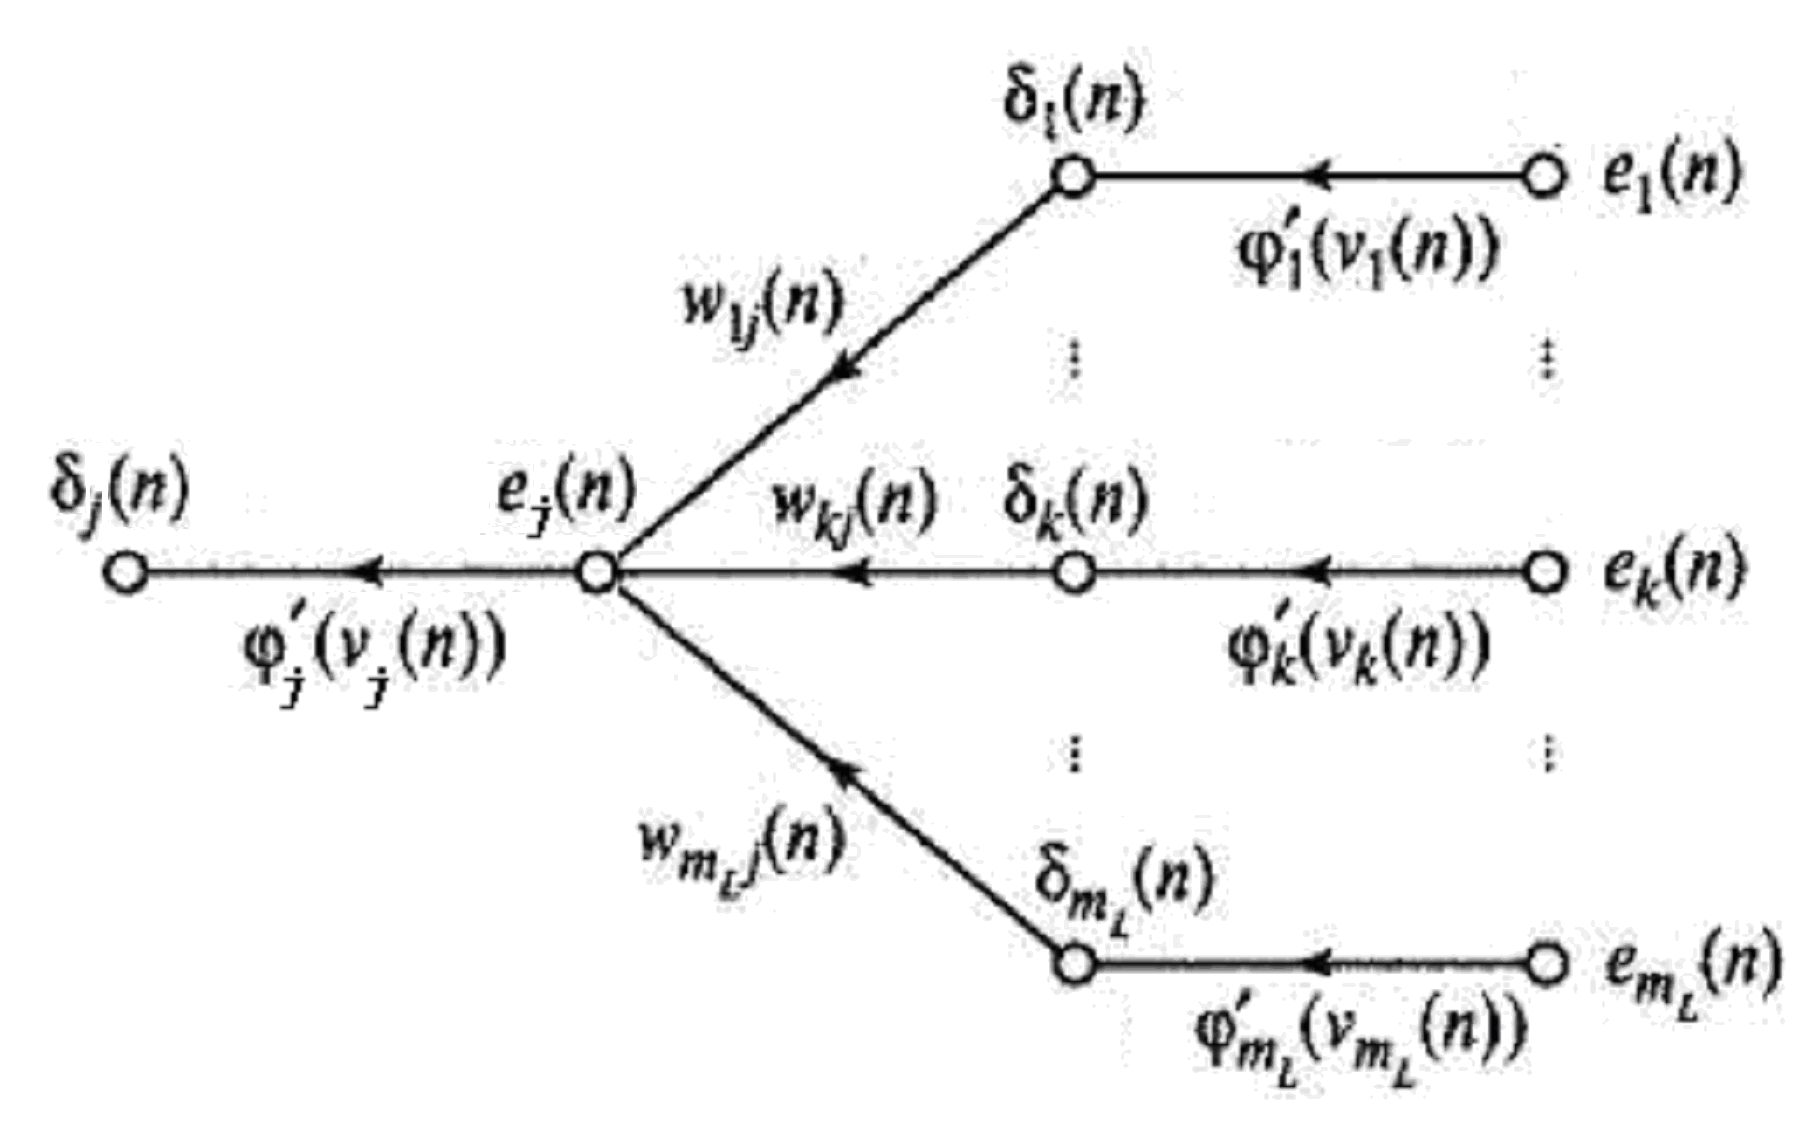
\includegraphics[height=5cm]{lec_neuro_08_4_5.png}
    \caption{Направление двух потоков сигналов в многослойном перцептроне}
    \label{lec_neuro_08_4_5}
\end{figure}

Основной результат заключается в правиле вычисления ошибок для нейронов младшего слоя. 
Показано, что сигнал ошибки может быть вычислен в виде взвешенной суммы локальных градиентов
нейронов n-го слоя: (4.24 ворд)

\begin{equation}
    e_j(n) = \sum_{k=1}^{m_3} w_{kj}(n) \delta_k (n)
\end{equation}

\begin{myquote}
    \textit{Возможно, суммирование должно быть от 0.}
\end{myquote}

Вычислив ошибку для нейронов второго слоя, вычислим для него локальный градиент, т.е. 
распространим ошибку на шаг назад:

\begin{equation}
    \delta_j(n) = e_j(n) \cdot \varphi^{\prime} (v_j(n))
\end{equation}

Значит, возможно произвести "редактирование" синаптических весов нейронов второго слоя. Т.е.:

\begin{equation}
    w_{ji}(n) = w_{ji}(n-1) + \dfrac{\eta}{N} \cdot \delta_j \cdot y_i(n)
\end{equation}

Для нейронов первого скрытого слоя:

\begin{equation}
    e_i(n) = \sum_{j=1}^{m_2} w_{ji}(n) \delta_j
\end{equation}

\begin{myquote}
    \textit{Возможно, суммирование должно быть от 0.}
\end{myquote}

\begin{equation}
    \delta_i(n) = e_i(n) \cdot \varphi^{\prime} (v_i(n))
\end{equation}

Для входного слоя получим:

\begin{equation}
    w_{il}(n) = w_{il}(n-1) + \dfrac{\eta}{N} \cdot \delta_i \cdot x_l
\end{equation}

Произошло распространение ошибок и локального градиента в обратном направлении, что
позволило применить обычное дельта-правило.




\section{Новая}
\subsection{Практические рекомендации по улучшению сходимости алгоритма обратного распространения ошибок}


\end{document}